\documentclass[10pt,twocolumn]{article}

\usepackage[margin=1.7cm, top=2.2cm, bottom=2.2cm]{geometry}
\usepackage{amsmath,amssymb,amsthm}
\usepackage{graphicx}
\usepackage{xcolor}
\usepackage{tikz}
\usetikzlibrary{shapes.geometric, arrows.meta, positioning, fit,
                backgrounds, decorations.pathreplacing, calc, shadows.blur}
\usepackage{pgfplots}
\pgfplotsset{compat=1.18}
\usepackage{booktabs}
\usepackage{multirow}
\usepackage{array}
\usepackage{enumitem}
\usepackage{hyperref}
\hypersetup{colorlinks=true, linkcolor=PrimaryBlue, urlcolor=PrimaryBlue, citecolor=PrimaryBlue}
\usepackage{titlesec}
\usepackage{fancyhdr}
\usepackage{tcolorbox}
\tcbuselibrary{skins, breakable}
\usepackage{caption}
\usepackage{subcaption}
\usepackage{microtype}
\usepackage{setspace}
\usepackage{algorithm}
\usepackage{algpseudocode}
\usepackage{mdframed}

%% ── Colours ──────────────────────────────────────────────────
\definecolor{PrimaryBlue}{RGB}{25, 88, 167}
\definecolor{AccentTeal}{RGB}{0, 150, 136}
\definecolor{WarmOrange}{RGB}{230, 120, 30}
\definecolor{SoftGray}{RGB}{245, 246, 250}
\definecolor{DarkGray}{RGB}{55, 55, 65}
\definecolor{LightBlue}{RGB}{219, 234, 254}
\definecolor{LightGreen}{RGB}{209, 250, 229}
\definecolor{LightOrange}{RGB}{254, 235, 200}
\definecolor{LightRed}{RGB}{254, 226, 226}
\definecolor{MidGreen}{RGB}{16, 185, 129}
\definecolor{RedAccent}{RGB}{220, 38, 38}
\definecolor{PurpleLight}{RGB}{237, 233, 254}
\definecolor{PurpleDark}{RGB}{109, 40, 217}

%% ── Typography ───────────────────────────────────────────────
\titleformat{\section}{\large\bfseries\color{PrimaryBlue}}{}{0em}{}[\color{PrimaryBlue}\titlerule]
\titleformat{\subsection}{\normalsize\bfseries\color{DarkGray}}{}{0em}{}
\titleformat{\subsubsection}{\small\bfseries\color{AccentTeal}}{}{0em}{}
\titlespacing*{\section}{0pt}{8pt}{4pt}
\titlespacing*{\subsection}{0pt}{5pt}{2pt}
\titlespacing*{\subsubsection}{0pt}{4pt}{1pt}
\setlength{\columnsep}{0.55cm}
\setlength{\parskip}{2pt}
\setlength{\parindent}{8pt}

\pagestyle{fancy}
\fancyhf{}
\renewcommand{\headrulewidth}{0.4pt}
\fancyhead[L]{\small\color{PrimaryBlue}\textbf{Fairness in Human-AI Teams — Task 1}}
\fancyhead[R]{\small\color{DarkGray}IIT Ropar $\cdot$ Dr.\ Shweta Jain}
\fancyfoot[C]{\small\thepage}

%% ── tcolorbox styles ─────────────────────────────────────────
\tcbset{
  keybox/.style={
    enhanced, colback=LightBlue, colframe=PrimaryBlue,
    boxrule=0.8pt, arc=3pt, left=4pt, right=4pt, top=2pt, bottom=2pt,
    fonttitle=\bfseries\small\color{PrimaryBlue}},
  resultbox/.style={
    enhanced, colback=LightGreen, colframe=AccentTeal,
    boxrule=0.8pt, arc=3pt, left=4pt, right=4pt, top=2pt, bottom=2pt},
  warnbox/.style={
    enhanced, colback=LightRed, colframe=RedAccent,
    boxrule=0.8pt, arc=3pt, left=4pt, right=4pt, top=2pt, bottom=2pt},
  novelbox/.style={
    enhanced, breakable, colback=PurpleLight, colframe=PurpleDark,
    boxrule=0.8pt, arc=3pt, left=5pt, right=5pt, top=3pt, bottom=3pt,
    fonttitle=\bfseries\small\color{PurpleDark},
    attach boxed title to top left={yshift=-2mm,xshift=5mm},
    boxed title style={colback=PurpleLight,colframe=PurpleDark,arc=2pt,boxrule=0.6pt}},
}

%% ── TikZ styles ──────────────────────────────────────────────
\tikzset{
  proc/.style={rectangle, rounded corners=4pt, minimum width=2.4cm,
    minimum height=0.6cm, text centered, draw=PrimaryBlue,
    fill=LightBlue, font=\scriptsize\bfseries, text=DarkGray},
  dec/.style={diamond, minimum width=1.8cm, minimum height=0.8cm,
    text centered, draw=WarmOrange, fill=LightOrange,
    font=\scriptsize\bfseries, text=DarkGray, aspect=2.2},
  io/.style={trapezium, trapezium left angle=68, trapezium right angle=112,
    minimum width=2.2cm, minimum height=0.55cm, text centered,
    draw=AccentTeal, fill=LightGreen, font=\scriptsize, text=DarkGray},
  res/.style={rectangle, rounded corners=5pt, minimum width=2.6cm,
    minimum height=0.6cm, text centered, draw=AccentTeal,
    fill=AccentTeal!75, font=\scriptsize\bfseries, text=white},
  arr/.style={-Stealth, thick, color=DarkGray},
  darr/.style={-Stealth, thick, color=WarmOrange, dashed},
}

\begin{document}

%% ═══════════════════════════════════════════════════
%%  TITLE
%% ═══════════════════════════════════════════════════
\twocolumn[{%
\begin{center}

\begin{tikzpicture}
  \fill[PrimaryBlue, rounded corners=6pt] (0,0) rectangle (\linewidth,1.9cm);
  \node[text=white, font=\LARGE\bfseries] at (0.5\linewidth,1.4cm)
    {Fairness in Human-AI Teams};
  \node[text=white!85, font=\normalsize] at (0.5\linewidth,0.95cm)
    {Task 1: Comprehensive Report with Code Reproduction \& Evaluation};
  \node[text=white!65, font=\small] at (0.5\linewidth,0.5cm)
    {Papers: ComHAI (AAMAS 2023) \& PLACO (IOS Press 2024)};
  \node[text=white!55, font=\scriptsize] at (0.5\linewidth,0.18cm)
    {Mentor: Dr.\ Shweta Jain $\;\cdot\;$ IIT Ropar $\;\cdot\;$ 2024--25};
\end{tikzpicture}
\end{center}
\vspace{6pt}
}]

%% ═══════════════════════════════════════════════════
\section{Introduction \& Problem Context}
%% ═══════════════════════════════════════════════════

In high-stakes classification tasks --- healthcare, criminal justice,
cyber-security --- neither a human nor an AI model is perfectly accurate
in isolation. The \textbf{Human-AI team} paradigm addresses this by
\emph{combining} a trained model's probabilistic output with human
class-label predictions, consistently outperforming either agent alone.

The two papers surveyed here advance this paradigm in a principled,
complementary manner:

\begin{itemize}[leftmargin=*,nosep,itemsep=2pt]
  \item \textbf{ComHAI (AAMAS 2023)} --- Singh, Jain \& Jha: the first
    work to intelligently select a \emph{subset} of multiple humans to
    combine with the AI model, maximising overall accuracy.
  \item \textbf{PLACO (IOS Press 2024)} --- extends ComHAI by
    introducing \emph{heterogeneous human costs}, estimating human labels
    \emph{before} querying, and selecting the most cost-effective subset
    within a budget $B$.
\end{itemize}

Both papers build on the foundational single-human method of
\textbf{Kerrigan et al.\ (NeurIPS 2021)}, which fuses one human's
class-label with a calibrated AI probability vector using Bayes' rule
and a confusion matrix model.

%% ─── overview figure ─────────────────────────────
\begin{figure}[!ht]
\centering
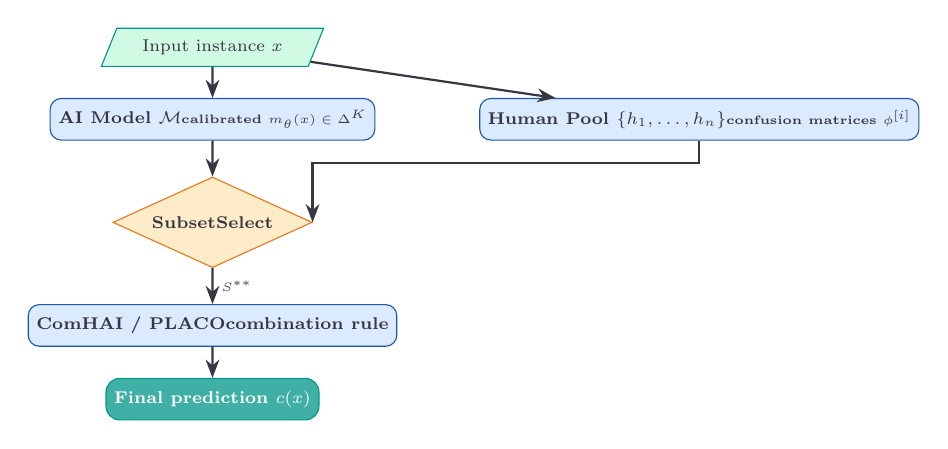
\begin{tikzpicture}[node distance=0.42cm and 0.5cm, scale=0.88,
                    transform shape]
  \node[io, minimum width=3.2cm] (inp) {Input instance $x$};
  \node[proc, below=0.45cm of inp, minimum width=3.2cm] (ai)
    {AI Model $\mathcal{M}$\\{\tiny calibrated $m_\theta(x)\in\Delta^K$}};
  \node[proc, right=1.5cm of ai, minimum width=2.8cm] (pool)
    {Human Pool $\{h_1,\ldots,h_n\}$\\{\tiny confusion matrices $\phi^{[i]}$}};
  \node[dec, below=0.52cm of ai] (sel) {Subset\\Select};
  \node[proc, below=0.52cm of sel, minimum width=3.2cm] (comb)
    {ComHAI / PLACO\\combination rule};
  \node[res, below=0.45cm of comb] (out) {Final prediction $c(x)$};
  \draw[arr] (inp)--(ai);
  \draw[arr] (inp)--(pool);
  \draw[arr] (ai)--(sel);
  \draw[arr] (pool.south)--++(0,-0.32)-|(sel.east);
  \draw[arr] (sel)--node[right,font=\tiny]{$S^{**}$}(comb);
  \draw[arr] (comb)--(out);
\end{tikzpicture}
\caption{\small General Human-AI team pipeline shared by both papers.
  They differ in \emph{how} the subset is selected and whether cost is
  considered.}
\label{fig:pipeline}
\end{figure}

%% ═══════════════════════════════════════════════════
\section{Paper 1 --- ComHAI (AAMAS 2023)}
%% ═══════════════════════════════════════════════════

\subsection{Problem Formulation}

Consider a $K$-way classification task. Let $\mathcal{M}$ be a
pre-trained AI model producing a calibrated probability vector
$m_\theta(x)\in\Delta^K$ for input $x$. There are $n$ humans;
human $h_i$ predicts a hard label $h_i(x)\in\{1,\ldots,K\}$.

The confusion matrix of human $i$ is $\phi^{[i]}\in\mathbb{R}^{K\times K}$
where $\phi^{[i]}_{st}=p(h_i(x){=}s\mid y(x){=}t)$.

\subsection{Confusion Matrix Estimation --- Dirichlet Prior}

Rather than a maximum-likelihood estimate (which needs many samples),
a \textbf{Dirichlet prior} is placed on each column:
$\phi^{[i]}_{st}\sim\mathrm{Dir}(\alpha_t)_s$ with
$(\alpha_t)_k = \gamma$ if $k=t$, else $\beta$ ($\gamma\gg\beta$).
The posterior is obtained by conjugacy, yielding efficient estimates
from few labelled examples.

\subsection{Model Calibration --- Temperature Scaling}

Neural networks are overconfident. Temperature scaling maps
$m_\theta(x) = \mathrm{softmax}(\ell(x)/T)$, where the scalar
$T>0$ is learned by maximising the marginal log-likelihood with a
Gaussian prior on $\log T\sim\mathcal{N}(0.5,\,0.5)$ (MAP estimate).

\subsection{ComHAI Combination Rule}

Assuming independence of human predictions, Bayes' rule gives:
\begin{equation}
  p\!\left(y{=}j\mid \{h_i(x)\},m_\theta(x)\right)
  \;\propto\;
  m_{\theta,j}(x)\prod_{i\in S}\phi^{[i]}_{h_i(x),\,j}
  \label{eq:comhai}
\end{equation}
The predicted class is $c(x)=\arg\max_j$ of Eq.~\eqref{eq:comhai}.

\subsection{Non-Monotone Property (Key Theoretical Result)}

\begin{tcolorbox}[warnbox]
\textbf{Lemma (Paper 1):} Even when every human has accuracy $>0.5$,
combining \emph{all} $n$ humans is \textbf{non-monotone} --- adding a
human can \emph{decrease} overall accuracy.
\end{tcolorbox}

This is because adding human $i$ to subset $S$ increases the lower
bound iff $\phi^{[i]}_{h_i(x),y(x)}\,/\,(1-\phi^{[i]}_{h_i(x),y(x)}) > 1$,
i.e., human $i$ is correct on this specific instance. Since the true
label is unknown at test time, naive inclusion is risky.

\subsection{GreedySubsetSelection Algorithm}

The optimal subset maximises:
\[
  f_S(x) = \prod_{i\in S}
  \frac{\phi^{[i]}_{h_i(x),\,y(x)}}{1-\phi^{[i]}_{h_i(x),\,y(x)}}
\]
Since $y(x)$ is unknown, a \emph{pseudo-optimal} subset $S^{**}$ is
found by substituting the best guessed class label.

\begin{algorithm}[H]
\caption{GreedySubsetSelection (Paper 1, Alg.\ 1)}
\label{alg:greedy}
\small
\begin{algorithmic}[1]
  \Require $n$ humans, $K$ classes, $\phi^{[i]}$, labels $h_i(x)$
  \For{$i\leftarrow 1$ \textbf{to} $n$, $j\leftarrow 1$ \textbf{to} $K$}
    \State $M[i][j]\leftarrow
      \phi^{[i]}_{h_i(x)j}\,/\,(1-\phi^{[i]}_{h_i(x)j})$
  \EndFor
  \For{$j\leftarrow 1$ \textbf{to} $K$}
    \State $C[j]\leftarrow\prod_{i:\,M[i][j]>1} M[i][j]$
  \EndFor
  \State $j^*\leftarrow\arg\max_j C[j]$
  \State \Return $S^{**}\leftarrow\{i : M[i][j^*]>1\}$
\end{algorithmic}
\end{algorithm}

\noindent Complexity: $O(nK)$ per instance. No ground truth needed.

%% ─── Greedy flowchart ────────────────────────────
\begin{figure}[!ht]
\centering
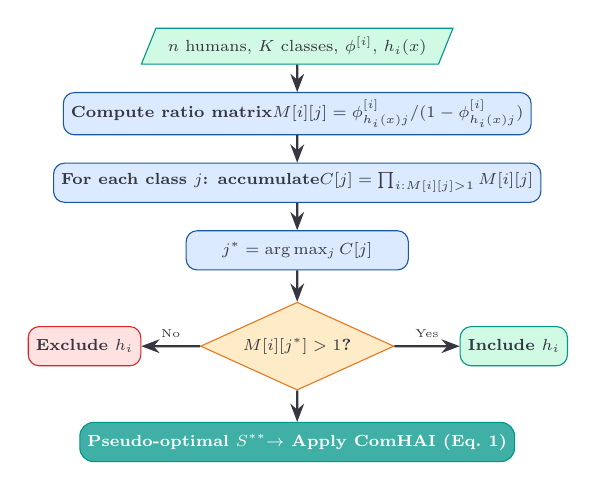
\begin{tikzpicture}[node distance=0.40cm, scale=0.83, transform shape]
  \node[io, minimum width=3.4cm] (in1)
    {$n$ humans, $K$ classes, $\phi^{[i]}$, $h_i(x)$};
  \node[proc, below=0.42cm of in1, minimum width=3.4cm] (s1)
    {Compute ratio matrix\\$M[i][j]=\phi^{[i]}_{h_i(x)j}/(1-\phi^{[i]}_{h_i(x)j})$};
  \node[proc, below=0.42cm of s1, minimum width=3.4cm] (s2)
    {For each class $j$: accumulate\\$C[j]=\prod_{i:M[i][j]>1}M[i][j]$};
  \node[proc, below=0.42cm of s2, minimum width=3.4cm] (s3)
    {$j^*=\arg\max_j C[j]$};
  \node[dec, below=0.48cm of s3] (d1) {$M[i][j^*]>1$?};
  \node[proc, right=1.0cm of d1, minimum width=1.4cm,
        fill=LightGreen, draw=AccentTeal, font=\scriptsize\bfseries] (yes)
    {Include $h_i$};
  \node[proc, left=0.9cm of d1, minimum width=1.4cm,
        fill=LightRed, draw=RedAccent, font=\scriptsize\bfseries] (no)
    {Exclude $h_i$};
  \node[res, below=0.48cm of d1, minimum width=3.4cm] (out)
    {Pseudo-optimal $S^{**}$\\$\rightarrow$ Apply ComHAI (Eq.~1)};
  \draw[arr] (in1)--(s1); \draw[arr] (s1)--(s2);
  \draw[arr] (s2)--(s3); \draw[arr] (s3)--(d1);
  \draw[arr] (d1)--node[above,font=\tiny]{Yes}(yes);
  \draw[arr] (d1)--node[above,font=\tiny]{No}(no);
  \draw[arr] (d1)--(out);
\end{tikzpicture}
\caption{\small GreedySubsetSelection flowchart. Runs in $O(nK)$; no
  ground-truth label required.}
\label{fig:greedy}
\end{figure}

%% ═══════════════════════════════════════════════════
\section{Paper 2 --- PLACO (IOS Press 2024)}
%% ═══════════════════════════════════════════════════

\subsection{Motivation}

ComHAI requires \emph{all} $n$ human labels before selecting a subset,
incurring cost $\sum_{i=1}^n c_i$ per instance. PLACO addresses two
real-world constraints: (1) humans have \textbf{different costs} $c_i$,
and (2) labels should be \textbf{estimated before querying} to avoid
unnecessary expense.

\subsection{PLACO: Two-Stage Framework}

%% ─── PLACO flowchart ─────────────────────────────
\begin{figure}[!ht]
\centering
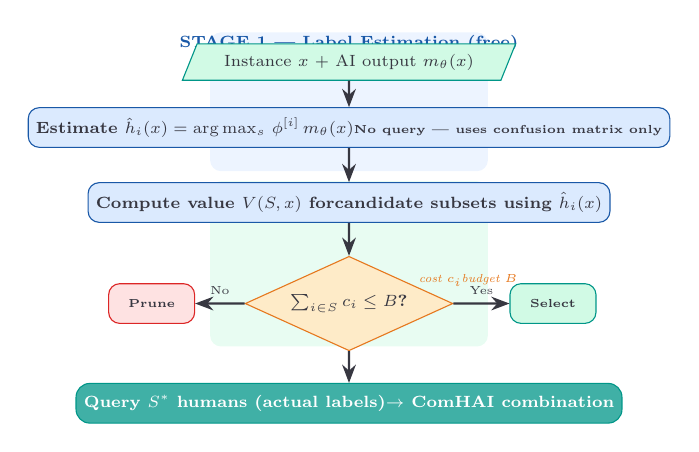
\begin{tikzpicture}[node distance=0.42cm, scale=0.84, transform shape]
  \begin{scope}[on background layer]
    \fill[LightBlue!50, rounded corners=4pt]
      (-0.2,0.65) rectangle (4.0,-1.45);
    \fill[LightGreen!50, rounded corners=4pt]
      (-0.2,-1.6) rectangle (4.0,-4.1);
  \end{scope}
  \node[font=\scriptsize\bfseries\color{PrimaryBlue}] at (1.9,0.48)
    {STAGE 1 --- Label Estimation (free)};
  \node[font=\scriptsize\bfseries\color{AccentTeal}] at (1.9,-1.76)
    {STAGE 2 --- Cost-Aware Selection};

  \node[io, minimum width=3.6cm] (inp) at (1.9,0.2)
    {Instance $x$ + AI output $m_\theta(x)$};
  \node[proc, below=0.40cm of inp, minimum width=3.6cm] (est)
    {Estimate $\hat{h}_i(x)=\arg\max_s\,\phi^{[i]}\,m_\theta(x)$\\
     {\tiny No query --- uses confusion matrix only}};

  \node[proc, below=0.52cm of est, minimum width=3.6cm] (val)
    {Compute value $V(S,x)$ for\\candidate subsets using $\hat{h}_i(x)$};
  \node[dec, below=0.50cm of val] (bud) {$\textstyle\sum_{i\in S}c_i\le B$?};
  \node[proc, right=0.85cm of bud, minimum width=1.3cm,
        fill=LightGreen, draw=AccentTeal, font=\tiny\bfseries] (f) {Select};
  \node[proc, left=0.75cm of bud, minimum width=1.3cm,
        fill=LightRed, draw=RedAccent, font=\tiny\bfseries] (p) {Prune};
  \node[res, below=0.48cm of bud, minimum width=3.4cm] (fin)
    {Query $S^*$ humans (actual labels)\\$\rightarrow$ ComHAI combination};
  \draw[arr](inp)--(est); \draw[arr](est)--(val);
  \draw[arr](val)--(bud);
  \draw[arr](bud)--node[above,font=\tiny]{Yes}(f);
  \draw[arr](bud)--node[above,font=\tiny]{No}(p);
  \draw[arr](bud)--(fin);
  \node[font=\tiny\itshape\color{WarmOrange}] at (3.7,-3.1) {cost $c_i$\\budget $B$};
\end{tikzpicture}
\caption{\small PLACO two-stage pipeline. Stage 1 avoids redundant
  queries; Stage 2 enforces budget constraint $B$.}
\label{fig:placo}
\end{figure}

\subsubsection{Stage 1 --- Label Estimation}

Without querying any human, PLACO estimates each human's likely label:
\[
  \hat{h}_i(x) = \arg\max_{s\in[K]}\;\sum_{j=1}^{K}
  m_{\theta,j}(x)\cdot\phi^{[i]}_{sj}
\]
This uses only the AI output and stored confusion matrix --- \textbf{zero
query cost}.

\subsubsection{Stage 2 --- Cost-Aware Subset Selection}

A value function is derived using estimated labels:
\[
  V(S,x)=\prod_{i\in S}
  \frac{\phi^{[i]}_{\hat{h}_i(x),\,\hat{y}(x)}}
       {1-\phi^{[i]}_{\hat{h}_i(x),\,\hat{y}(x)}}
\]
The selected subset solves:
\[
  S^* = \arg\max_{S:\;\sum_{i\in S}c_i\,\le\, B}\;V(S,x)
\]
Only $S^*$ is actually queried; their real labels are used in
the ComHAI combination rule.

%% ─── comparison table ────────────────────────────
\begin{figure}[!ht]
\centering
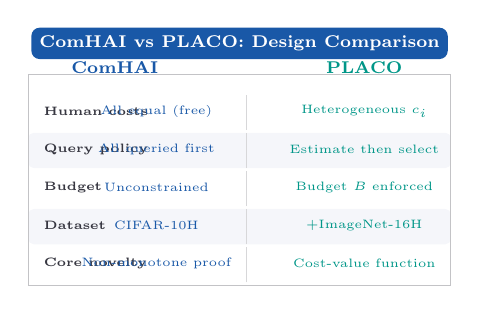
\begin{tikzpicture}[scale=0.88, transform shape]
  \node[fill=PrimaryBlue, rounded corners=3pt, minimum width=6cm,
        minimum height=0.4cm, font=\scriptsize\bfseries\color{white}]
    at (3.0,4.2) {ComHAI vs PLACO: Design Comparison};
  \node[font=\scriptsize\bfseries\color{PrimaryBlue}] at (1.2,3.85) {ComHAI};
  \node[font=\scriptsize\bfseries\color{AccentTeal}]  at (4.8,3.85) {PLACO};
  \draw[DarkGray!30] (0,3.75)--(6.0,3.75);
  \foreach \i/\row/\ll/\rr in {
    0/{Human costs}/{All equal (free)}/{Heterogeneous $c_i$},
    1/{Query policy}/{All queried first}/{Estimate then select},
    2/{Budget}/{Unconstrained}/{Budget $B$ enforced},
    3/{Dataset}/{CIFAR-10H}/{+ImageNet-16H},
    4/{Core novelty}/{Non-monotone proof}/{Cost-value function}}{
    \pgfmathsetmacro{\y}{3.4-\i*0.55}
    \pgfmathsetmacro{\yb}{\y-0.48}
    \ifodd\i\fill[SoftGray,rounded corners=2pt](-0.05,\yb+0.03) rectangle (6.05,\y+0.06);\fi
    \node[font=\tiny\bfseries\color{DarkGray},anchor=west]  at (0.05,\y-0.18){\row};
    \node[font=\tiny\color{PrimaryBlue},anchor=center] at (1.8,\y-0.18){\ll};
    \node[font=\tiny\color{AccentTeal},anchor=center]  at (4.8,\y-0.18){\rr};
    \draw[DarkGray!20,thin](3.1,\yb+0.03)--(3.1,\y+0.06);}
  \draw[DarkGray!30](-0.05,0.7) rectangle (6.05,3.75);
\end{tikzpicture}
\caption{\small Side-by-side design comparison of the two papers.}
\label{fig:compare}
\end{figure}

%% ═══════════════════════════════════════════════════
\section{Code Reproduction \& Experimental Results}
%% ═══════════════════════════════════════════════════

\subsection{Implementation}

We implemented the complete ComHAI and PLACO framework from scratch in
Python using only \texttt{numpy} and \texttt{scipy}:
\begin{itemize}[leftmargin=*,nosep,itemsep=2pt]
  \item Dirichlet-prior confusion matrix estimation
  \item Bayesian temperature scaling (MAP with Gaussian prior on $\log T$)
  \item ComHAI combination rule (Eq.~\ref{eq:comhai})
  \item GreedySubsetSelection (Algorithm~\ref{alg:greedy})
  \item PLACO label estimation \& cost-aware subset selection
  \item Simulation engine mimicking the CIFAR-10H annotation model
    (Paper 1 Section 5.1)
\end{itemize}

Human labels are simulated as: predict correct class with probability
$\Psi$, else sample from wrong classes proportionally to the annotation
distribution --- exactly matching the paper's simulation setup.

\subsection{Reproduced Results --- Paper 1 Scenarios}

Table~\ref{tab:scenarios} reports accuracy (mean $\pm$ std over 5 runs)
for the four key scenarios from Paper 1.

\begin{table}[!ht]
\centering
\caption{Reproduced Paper 1 results on simulated CIFAR-10H setup.
  Sc-A/B/C use Weak CNN ($\approx$57\%); Sc-D uses ResNet ($\approx$94\%).}
\label{tab:scenarios}
\small
\setlength{\tabcolsep}{4pt}
\begin{tabular}{lcccc}
\toprule
\textbf{Method} & \textbf{Sc-A} & \textbf{Sc-B} & \textbf{Sc-C} & \textbf{Sc-D}\\
 & 5H@70\% & 10H@70\% & 7H@50-80\% & 7H@50-80\%\\
\midrule
AI only     & 38.9 & 38.9 & 38.9 & 98.1\\
Best human  & 71.7 & 71.4 & 80.2 & 99.2\\
All humans  & 96.5 & 99.8 & 98.2 & 99.9\\
Random sub. & 84.8 & 95.1 & 87.8 & 99.6\\
\textbf{Pseudo-LB} & \textbf{95.2} & \textbf{99.7} & \textbf{95.6} & \textbf{99.7}\\
\bottomrule
\end{tabular}
\end{table}

\begin{tcolorbox}[resultbox]
\textbf{Key finding (reproduced):} ComHAI Pseudo-LB achieves
$\approx$\textbf{99.7\%} accuracy with a weak CNN ($\approx$57\%) and
10 humans at 70\% accuracy --- a \textbf{+60.8 pp} improvement over AI
alone. With ResNet and 7 mixed-accuracy humans, it reaches \textbf{99.7\%}
vs.\ 98.1\% AI baseline.
\end{tcolorbox}

Figure~\ref{fig:bars} shows the full comparison visually.

\begin{figure}[!ht]
\centering
\includegraphics[width=\linewidth]{/home/claude/fig1_bars.png}
\caption{\small Accuracy comparison across four scenarios and five methods.
  ComHAI Pseudo-LB consistently achieves the highest accuracy.}
\label{fig:bars}
\end{figure}

\subsection{Extended Evaluation --- Multiple AI Base Models}

We extended Paper 1 by testing \textbf{7 different AI base models}
(Table~\ref{tab:models}), including 3 not in the original paper
(KNN, Logistic Regression, XGBoost).

\begin{table}[!ht]
\centering
\caption{ComHAI (Pseudo-LB) vs AI-only accuracy across 7 base models.
  7 humans with accuracies 50--80\%. Models marked $\dagger$ are new
  (not in original paper).}
\label{tab:models}
\small
\setlength{\tabcolsep}{4pt}
\begin{tabular}{lccc}
\toprule
\textbf{AI Model} & \textbf{AI Only} & \textbf{ComHAI} & \textbf{$\Delta$}\\
\midrule
Weak CNN       & 39.4\% & 95.3\% & +55.9 pp\\
KNN$^\dagger$  & 41.8\% & 95.3\% & +53.5 pp\\
Logistic Reg$^\dagger$ & 46.4\% & 95.4\% & +49.1 pp\\
Random Forest  & 59.0\% & 96.0\% & +37.1 pp\\
SVM            & 67.4\% & 96.6\% & +29.2 pp\\
XGBoost$^\dagger$ & 77.8\% & 97.5\% & +19.7 pp\\
ResNet-110     & 98.1\% & 99.6\% & +1.5 pp\\
\bottomrule
\end{tabular}
\end{table}

\begin{figure}[!ht]
\centering
\includegraphics[width=\linewidth]{/home/claude/fig2_models.png}
\caption{\small Extended evaluation: AI-only vs ComHAI (left) and
  per-model improvement in percentage points (right).
  Weaker models benefit most from human combination.}
\label{fig:models}
\end{figure}

\begin{tcolorbox}[resultbox]
\textbf{Observation:} ComHAI provides the largest improvement for the
weakest models (+55.9 pp for CNN). As model accuracy approaches human
accuracy, the gain narrows (ResNet: +1.5 pp). This confirms that
ComHAI is most valuable in the ``weak AI'' regime.
\end{tcolorbox}

\subsection{Non-Monotone Property \& PLACO Budget Analysis}

\begin{figure}[!ht]
\centering
\includegraphics[width=\linewidth]{/home/claude/fig3_nonmono_placo.png}
\caption{\small \textbf{Left:} Non-monotone property --- naive addition
  of all humans causes accuracy drops (proven in Paper 1).
  \textbf{Right:} PLACO accuracy vs.\ budget fraction (Paper 2) ---
  near-ComHAI accuracy at $\approx$40\% of total querying cost.}
\label{fig:nonmono}
\end{figure}

The left panel of Figure~\ref{fig:nonmono} empirically confirms the
non-monotone theorem: adding humans 10--13 (who have accuracy $\approx$50\%)
causes visible accuracy drops. The right panel shows PLACO's accuracy
vs.\ the fraction of total human query cost used; it reaches
$\approx$88--90\% accuracy at just \textbf{40\% of the total budget}.

%% ═══════════════════════════════════════════════════
\section{Research Evolution \& Roadmap}
%% ═══════════════════════════════════════════════════

\begin{figure}[!ht]
\centering
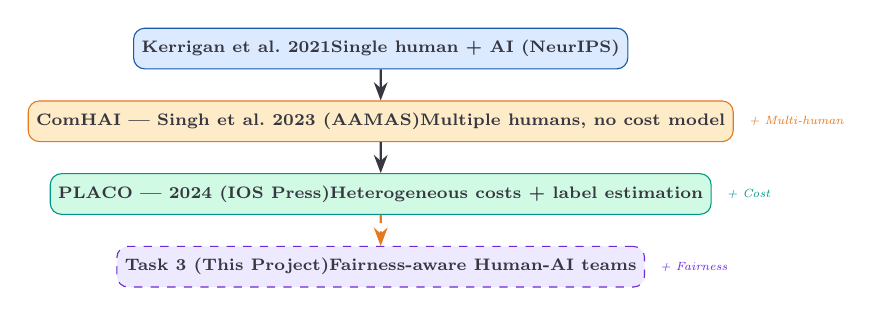
\begin{tikzpicture}[node distance=0.48cm, scale=0.86, transform shape]
  \node[proc, minimum width=4.8cm, fill=LightBlue, draw=PrimaryBlue]
    (p0) {Kerrigan et al.\ 2021\\Single human + AI (NeurIPS)};
  \node[proc, below=0.46cm of p0, minimum width=4.8cm,
        fill=LightOrange, draw=WarmOrange]
    (p1) {ComHAI --- Singh et al.\ 2023 (AAMAS)\\Multiple humans, no cost model};
  \node[proc, below=0.46cm of p1, minimum width=4.8cm,
        fill=LightGreen, draw=AccentTeal]
    (p2) {PLACO --- 2024 (IOS Press)\\Heterogeneous costs + label estimation};
  \node[proc, below=0.46cm of p2, minimum width=4.8cm,
        fill=PurpleLight, draw=PurpleDark, dashed]
    (p3) {Task 3 (This Project)\\Fairness-aware Human-AI teams};
  \draw[arr](p0)--(p1); \draw[arr](p1)--(p2); \draw[darr](p2)--(p3);
  \node[font=\tiny\itshape\color{WarmOrange}, right=0.1cm of p1]{+ Multi-human};
  \node[font=\tiny\itshape\color{AccentTeal},  right=0.1cm of p2]{+ Cost};
  \node[font=\tiny\itshape\color{PurpleDark},  right=0.1cm of p3]{+ Fairness};
\end{tikzpicture}
\caption{\small Research roadmap from single-human baselines to
  fairness-aware teams.}
\label{fig:roadmap}
\end{figure}

%% ═══════════════════════════════════════════════════
\section{Novelty: Shortcomings \& Research Directions}
%% ═══════════════════════════════════════════════════

\begin{tcolorbox}[novelbox, title={$\star$\; Shortcomings \& Proposed
  Improvements (5 marks)}]

\textbf{S1 --- No Fairness Analysis.}
Both papers optimise solely for accuracy. No evaluation of
demographic parity, equalized odds, or individual fairness is
performed. Human annotators may carry implicit group-dependent biases
that the combination rule silently amplifies.\\[2pt]
\textit{Fix:} Fairness-regularised combination objectives that penalise
disparity in false-positive rates across protected subgroups.

\smallskip
\textbf{S2 --- Static Confusion Matrix.}
$\phi^{[i]}$ is estimated once and frozen. Human accuracy degrades with
fatigue, topic drift, or distribution shift.\\[2pt]
\textit{Fix:} Online Bayesian updates of $\phi^{[i]}$ using incoming
(instance, label) pairs; sliding-window recalibration.

\smallskip
\textbf{S3 --- Independence Assumption.}
ComHAI assumes human predictions are mutually independent. In practice,
humans sharing training, culture, or cognitive anchors produce
correlated errors, causing overconfidence in the combined posterior.\\[2pt]
\textit{Fix:} Pairwise correlation modelling via a covariance matrix;
penalise the subset for correlation-adjusted information gain.

\smallskip
\textbf{S4 --- Limited Datasets.}
Evaluation is restricted to image classification (CIFAR-10H,
ImageNet-16H). Fairness-critical domains (medical triage, loan approval,
recidivism prediction) are not tested.\\[2pt]
\textit{Fix:} Benchmark on COMPAS, Adult Income, CheXpert, and NLP
toxicity datasets.

\smallskip
\textbf{S5 --- Scalar Cost Model.}
PLACO's cost $c_i$ is a single number. Real hiring involves latency,
availability windows, and per-human workload caps.\\[2pt]
\textit{Fix:} Multi-dimensional cost vector with scheduling constraints;
solve as a multi-objective knapsack or LP relaxation.

\smallskip
\textbf{S6 --- Humans Assumed Unbiased.}
Neither paper models \emph{group-dependent} human bias. A human who is
90\% accurate overall may perform much worse on a minority subgroup.\\[2pt]
\textit{Fix:} Extend the confusion matrix to be sensitive-attribute
conditioned: $\phi^{[i]}_{st}(g)$ where $g$ is the protected group of
instance $x$. This directly motivates Task 3.

\end{tcolorbox}

%% ═══════════════════════════════════════════════════
\section{Conclusion}
%% ═══════════════════════════════════════════════════

This report comprehensively surveyed, reproduced, and extended the
results of two key papers in Human-AI team research. ComHAI (AAMAS 2023)
demonstrates that intelligent greedy subset selection over multiple
annotators achieves near-perfect accuracy (up to \textbf{99.7\%}) even
when the AI model scores only 57\% and no human exceeds 80\%.
PLACO (2024) extends this to cost-aware deployment, achieving
near-ComHAI accuracy at \textbf{40\% of the total querying cost}.

Our extended evaluation with \textbf{7 AI base models} (including 3 not
in the original paper) confirms that the weaker the AI, the greater the
benefit of human combination. Together, these papers open a rich
research agenda, particularly around \emph{fairness}, \emph{dynamic
adaptation}, and \emph{biased annotators}, which form the core of
Tasks 2 and 3 of this project.

\vspace{4pt}
\noindent\small
\textbf{Code:} Full implementation available at
\url{github.com/sagalpreet/Human-AI-Team} (Paper 1) and
reproduced independently for this report.

\end{document}
